\documentclass[professionalfont]{beamer}

\usepackage{graphicx}
\usepackage{newtxtext,newtxmath}
\usepackage[backend=bibtex]{biblatex} 
\addbibresource{ref.bib}
\renewcommand*{\bibfont}{\scriptsize}

\usetheme{default}
\usecolortheme{seagull}

\setbeamertemplate{navigation symbols}{}
\setbeamertemplate{itemize item}{\textbullet} 
\setbeamertemplate{bibliography item}[text]
\setbeamertemplate{title page}{
    \begin{center}
        {\textcolor{blue}{\textbf{\fontsize{13}{14}\selectfont
        Language Models are Few-Shot Learners}}} \\[1.5cm]
        
        {\fontsize{9}{14}\selectfont Tom B. Brown, et al \\[0.3cm]
        OpenAI \\[0.3cm]
        NeurIPS 2020}
    \end{center}
}
% ------------------ Title ------------------

\begin{document}
\frame{\titlepage}

\begin{frame}
\begin{center}
    { \textbf{\textcolor{blue}{ {\fontsize{12}{14}\selectfont Abstract} }} }
\end{center}
\\[0.5cm]

{\fontsize{10}{14}\selectfont 
\begin{itemize}
    \item Task-specific
    
    - Different models for different tasks

    \\[0.3cm]

    \item Task agnostic (Fine-tuning)

    - One model fine-tuning for different tasks

    \\[0.3cm]

    \item Task agnostic (Prompting)

    - No weight update in the few-shot setting

    - We train GPT-3 with 175B parameters
\end{itemize}
}

\end{frame}
% ------------------ Slide 1 ------------------

\begin{frame}
\begin{center}
    { \textbf{\textcolor{blue}{ {\fontsize{12}{14}\selectfont Introduction} }} }
\end{center}

\begin{center}
    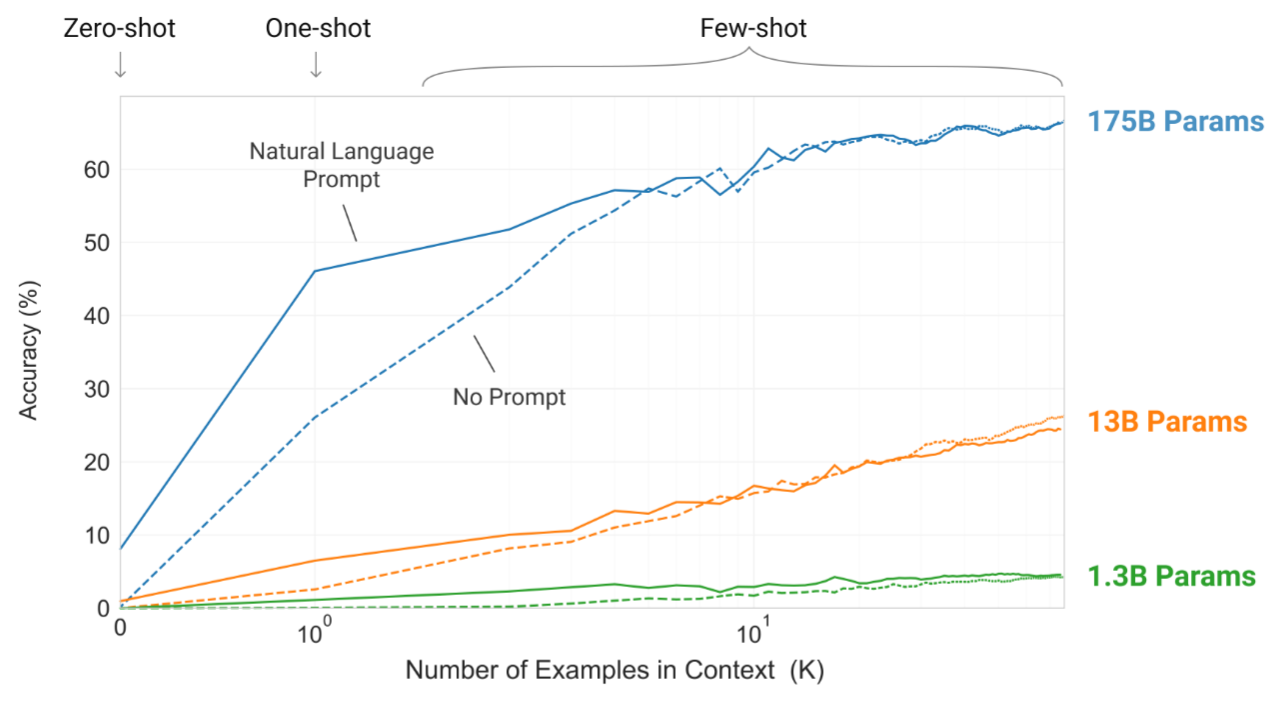
\includegraphics[width=0.8\textwidth]{figure/1-2.png}
\end{center}

{\fontsize{10}{14}\selectfont 
\begin{itemize}
    \item GPT-2 showed trend in performance and model size
    
    - However, it was zero-shot and far from supervised SOTA

    \\[0.3cm]

    \item We suggest GPT-3 with 175B parameters, few-shot settings

    - Larger models make efficient use of in-context information
    
\end{itemize}
}

\end{frame}
% ------------------ Slide 2 ------------------

\begin{frame}

\begin{center}
    { \textbf{\textcolor{blue}{ {\fontsize{12}{14}\selectfont Approach } }} }
\end{center}
\\[0.5cm]

{\fontsize{10}{14}\selectfont 
\begin{itemize}
    \item Fine-Tuning (FT)

    - Updates the weights with thousands of supervised labels
    
    \\[0.3cm]
    
    \item Few-Shot (FS)

    - K examples of context and completion are given
    
    \\[0.3cm]

    \item One-Shot (1S)

    - Similar to few-shot but with \( K = 1 \)
    
    \\[0.3cm]

    \item Zero-Shot (0S)

    - Natural language description of the task instead of examples
    
    \\[0.3cm]
\end{itemize}
}

\end{frame}
% ------------------ Slide 3 ------------------

\begin{frame}
\begin{refsection}

\begin{center}
    { \textbf{\textcolor{blue}{ {\fontsize{12}{14}\selectfont Model and Architectures} }} }
\end{center}

\begin{center}
    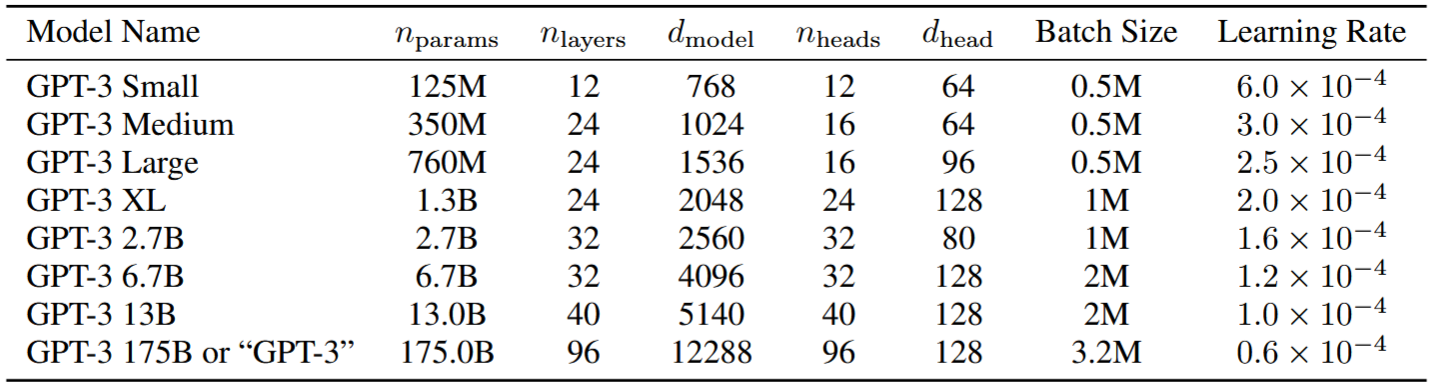
\includegraphics[width=1.0\textwidth]{table//2-1.png}
\end{center}

{\fontsize{10}{14}\selectfont 
\begin{itemize}
    \item Same model and architecture as GPT-2 \cite{gpt2}
    
    - Modified initialization and normalization

    - New feature: alternating dense sparse attention in the layers

    \item We train 8 different sizes of model

    - From 125M parameters to 175B parameters

    - Measured gradient noise scale to optimize hyperparameters
\end{itemize}
}

\vspace{0.2cm}
\hrule
\printbibliography

\end{refsection}
\end{frame}
% ------------------ Slide 4 ------------------

\begin{frame}
\begin{center}
    { \textbf{\textcolor{blue}{ {\fontsize{12}{14}\selectfont Training Dataset} }} }
\end{center}

\begin{center}
    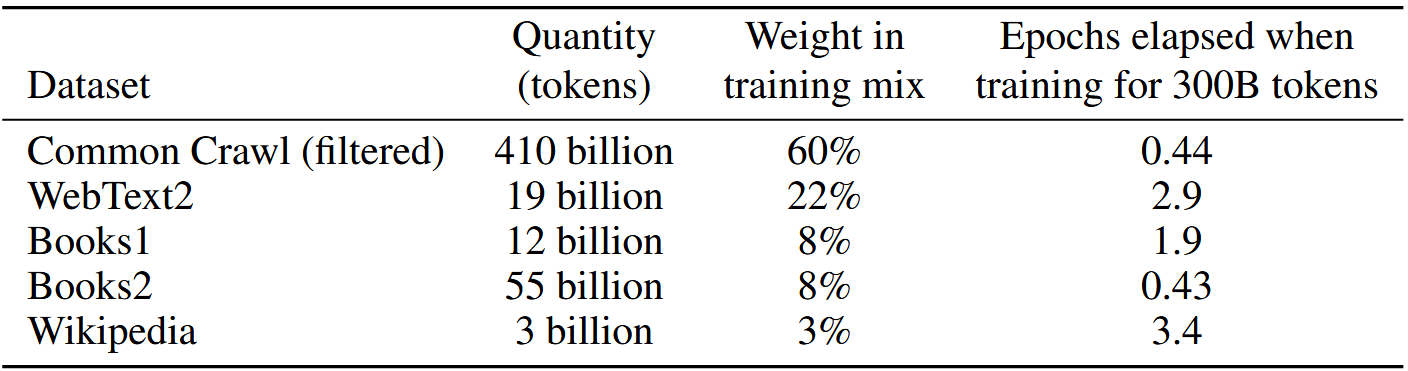
\includegraphics[width=1.0\textwidth]{table//2-2.png}
\end{center}

{\fontsize{10}{14}\selectfont 
\begin{itemize}
    \item Common Crawl dataset
    
    - Constituting nearly a trillion words

    - Low quality, which can degrade the performance

    \\[0.2cm]

    \item Improving Dataset Quality

    - Filtering based on similarity to high-quality  corpora

    - Fuzzy Deduplication to prevent overfitting

    - Added known high-quality reference corpora
\end{itemize}
}

\end{frame}
% ------------------ Slide 5 ------------------

\begin{frame}
\begin{center}
    { \textbf{\textcolor{blue}{ {\fontsize{12}{14}\selectfont Few-Shot Settings} }} }
\end{center}
\\[0.5cm]

{\fontsize{10}{14}\selectfont 
\begin{itemize}
    \item Give \( K \) examples from the task dataset

    - \( 0 \leq K \leq 2048 \) but typically \( 10 \leq K \leq 100 \) fits

    \\[0.2cm]

    \item Natural language prompt in addition to the examples

    - e.g., ``Translate this sentence:"

\end{itemize}
}

\end{frame}
% ------------------ Slide 6 ------------------

\begin{frame}
\begin{center}
    { \textbf{\textcolor{blue}{ {\fontsize{12}{14}\selectfont Task types} }} }
\end{center}
\\[0.3cm]

{\fontsize{10}{14}\selectfont 
\begin{itemize}
    \item Multiple-Choice Tasks

    - ARC, OpenBookQA, and RACE

    - It predicts the likelihood of each completion

    - Normalizing \( \frac{P(completion|context)}{P(completion|answer\_context)} \)

    - Answer context is ``Answer: "

    \\[0.2cm]

    \item Free-Form Completion Tasks

    - LAMBADA, TriviaQA, PiQA

    - Beam search: width of 4, length penalty \( \alpha = 0.6 \)

\end{itemize}
}

\end{frame}
% ------------------ Slide 7 ------------------

\begin{frame}
\begin{center}
    { \textbf{\textcolor{blue}{ {\fontsize{12}{14}\selectfont Experiment - LAMBADA} }} }
\end{center}

\begin{center}
    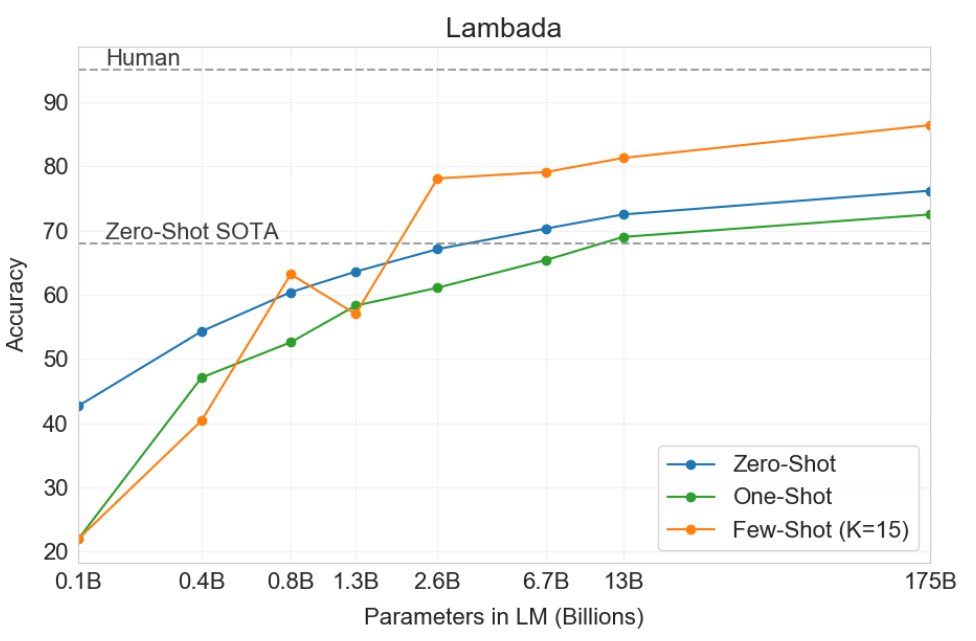
\includegraphics[width=0.7\textwidth]{figure/3-2.png}
\end{center}

{\fontsize{10}{14}\selectfont 
\begin{itemize}
    \item LAMBADA: Predicting last word of sentences

    - In recent studies, scaling up was not helpful on LAMBADA

    \item GPT-3 Results
    
    - GPT-3 showed significant improvements

\end{itemize}
}

\end{frame}
% ------------------ Slide 8 ------------------

\begin{frame}
\begin{center}
    { \textbf{\textcolor{blue}{ {\fontsize{12}{14}\selectfont Experiment - Story prediction} }} }
\end{center}
\\[0.5cm]

\begin{center}
    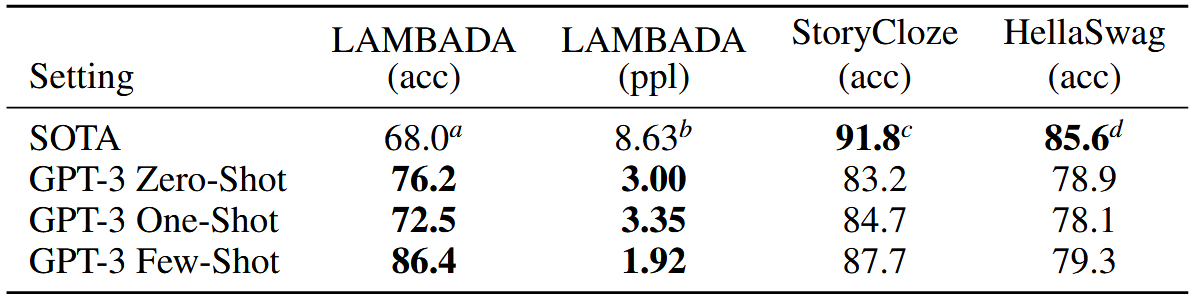
\includegraphics[width=1.0\textwidth]{table/3-2.png}
\end{center}

{\fontsize{10}{14}\selectfont 
\begin{itemize}
    \item HellaSwag

    - Slightly below the fine-tuned SOTA (ALUM)

    \\[0.3cm]

    \item StoryCloze
    
    - Slightly below the fine-tuned SOTA (BERT Based)

\end{itemize}
}

\end{frame}
% ------------------ Slide 9 ------------------

\begin{frame}
\begin{center}
    { \textbf{\textcolor{blue}{ {\fontsize{12}{14}\selectfont Experiment - Closed book QA} }} }
\end{center}

\begin{center}
    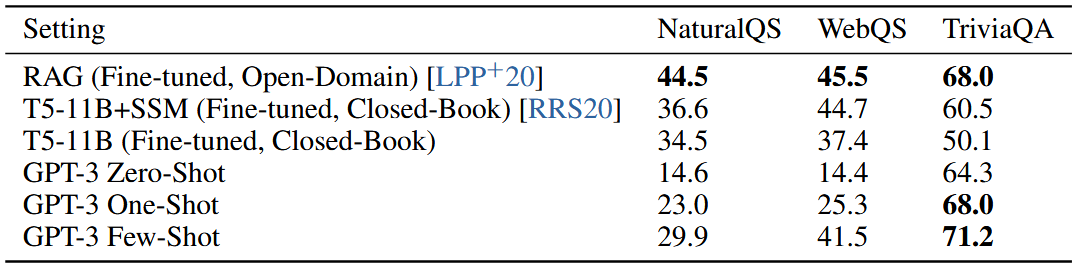
\includegraphics[width=1.0\textwidth]{table/3-3.png}
\end{center}

{\fontsize{10}{14}\selectfont 
\begin{itemize}
    \item NaturalQS: Real queries submitted to Google Search

    - Large gain from zero-shot to few-shot

    - Far from fine-tuned performace

    - Q\&A style may be out-of-distribution for GPT-3

    \item WebQS: Questions sourced from web queries
    
    - Close to RAG Performance

    \item TriviaQA: Focusing on fact-based questions
    
    - Outperformed fine-tuned models

\end{itemize}
}

\end{frame}
% ------------------ Slide 10 ------------------

\begin{frame}
\begin{center}
    { \textbf{\textcolor{blue}{ {\fontsize{12}{14}\selectfont Experiment - Translation} }} }
\end{center}

\begin{center}
    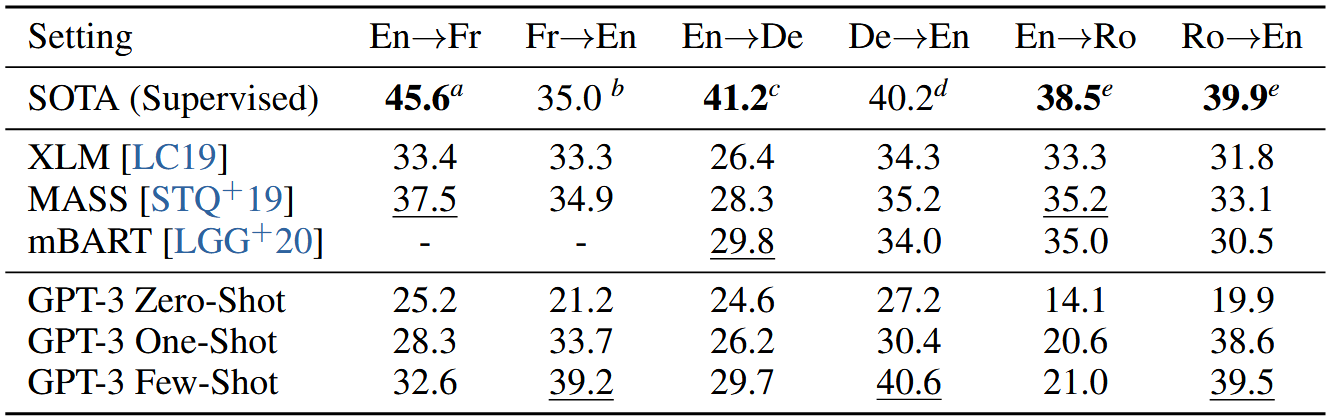
\includegraphics[width=1.0\textwidth]{table/3-4.png}
\end{center}

{\fontsize{10}{14}\selectfont 
\begin{itemize}
    \item 7\% of training data is non-English

    - In GPT-2, less than 0.1\% was French data

    - We expand translation to French, German, Romanian

    \item Language Directionality

    - Better performance when translating into English

    - Poor performance when translating from English

\end{itemize}
}

\end{frame}
% ------------------ Slide 11 ------------------

\begin{frame}

\begin{center}
    { \textbf{\textcolor{blue}{ {\fontsize{12}{14}\selectfont Experiment - Winograd Tasks} }} }
\end{center}

\begin{center}
    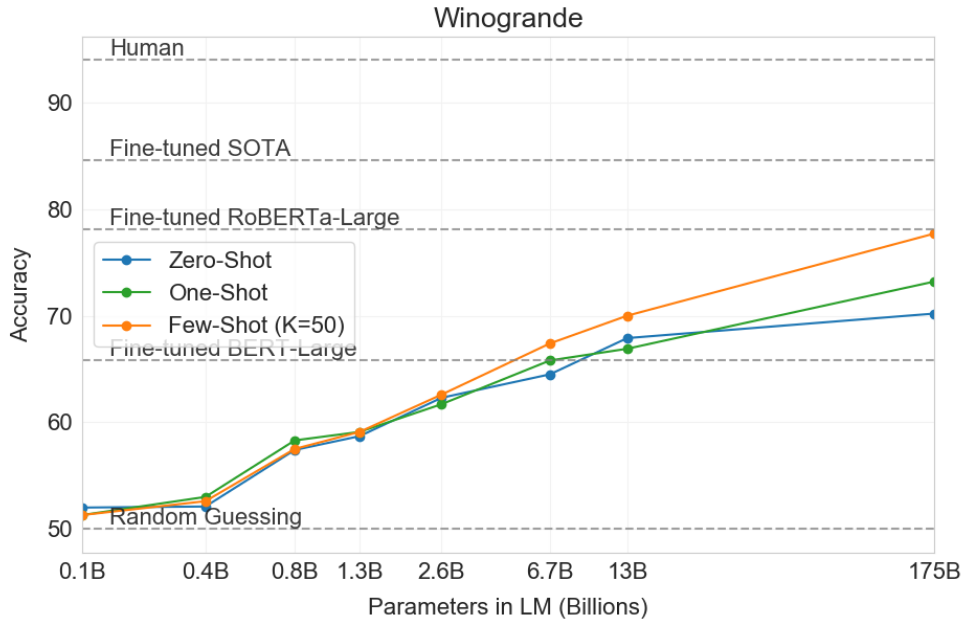
\includegraphics[width=0.9\textwidth]{figure/3-5.png}
\end{center}

{\fontsize{10}{14}\selectfont 
\begin{itemize}
    \item Significant gains from zero-shot to few-shot settings

    \item Still lags behind fine-tuned models and human performance

\end{itemize}
}

\end{frame}
% ------------------ Slide 12 ------------------

\begin{frame}

\begin{center}
    { \textbf{\textcolor{blue}{ {\fontsize{12}{14}\selectfont Experiment - Commonsense Reasoning} }} }
\end{center}

\begin{center}
    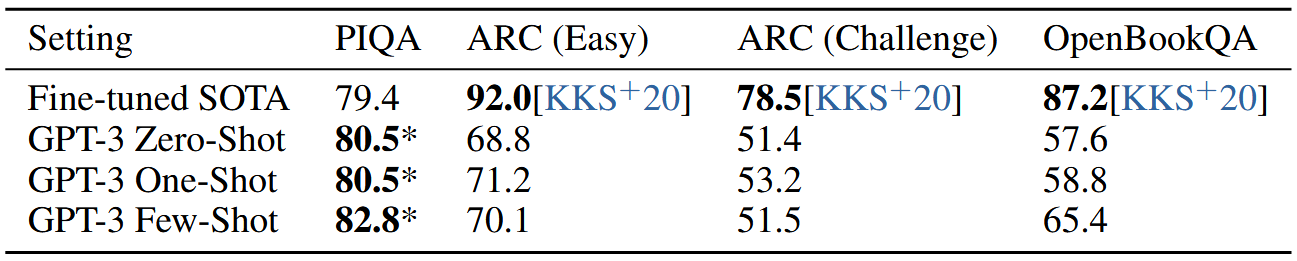
\includegraphics[width=0.9\textwidth]{table/3-6.png}
\end{center}

{\fontsize{10}{14}\selectfont 
\begin{itemize}
    \item PIQA (PhysicalQA)

    - Understanding of how the physical world works

    - ``How would you dry wet clothes faster?"

    \item ARC (AI2 Reasoning Challenge)

    - Multiple-choice science questions

    \item OpenBookQA

    - Reasoning about facts taught in elementary science class

    - ``Why do humans sweat?"

\end{itemize}
}

\end{frame}
% ------------------ Slide 13 ------------------

\begin{frame}

\begin{center}
    { \textbf{\textcolor{blue}{ {\fontsize{12}{14}\selectfont Experiment - Reading Comprehension} }} }
\end{center}
\\[0.2cm]

\begin{center}
    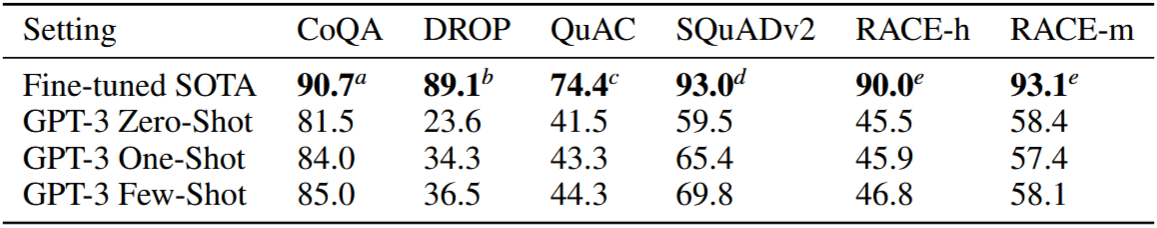
\includegraphics[width=1.0\textwidth]{table/3-7.png}
\end{center}

{\fontsize{10}{14}\selectfont 
\begin{itemize}
    \item Performs exceptionally well on CoQA

    - Free form text, which is in-context for GPT-3

    \\[0.2cm]

    \item Other datasets are more advanced

    - DROP requires numerical reasoning

    - QuAC has structured dialog and span selection

    - SQuAD includes unanswerable questions

    - RACE is multiple choice question in school

\end{itemize}
}

\end{frame}
% ------------------ Slide 14 ------------------

\begin{frame}

\begin{center}
    { \textbf{\textcolor{blue}{ {\fontsize{12}{14}\selectfont Experiment - SuperGLUE} }} }
\end{center}

\begin{center}
    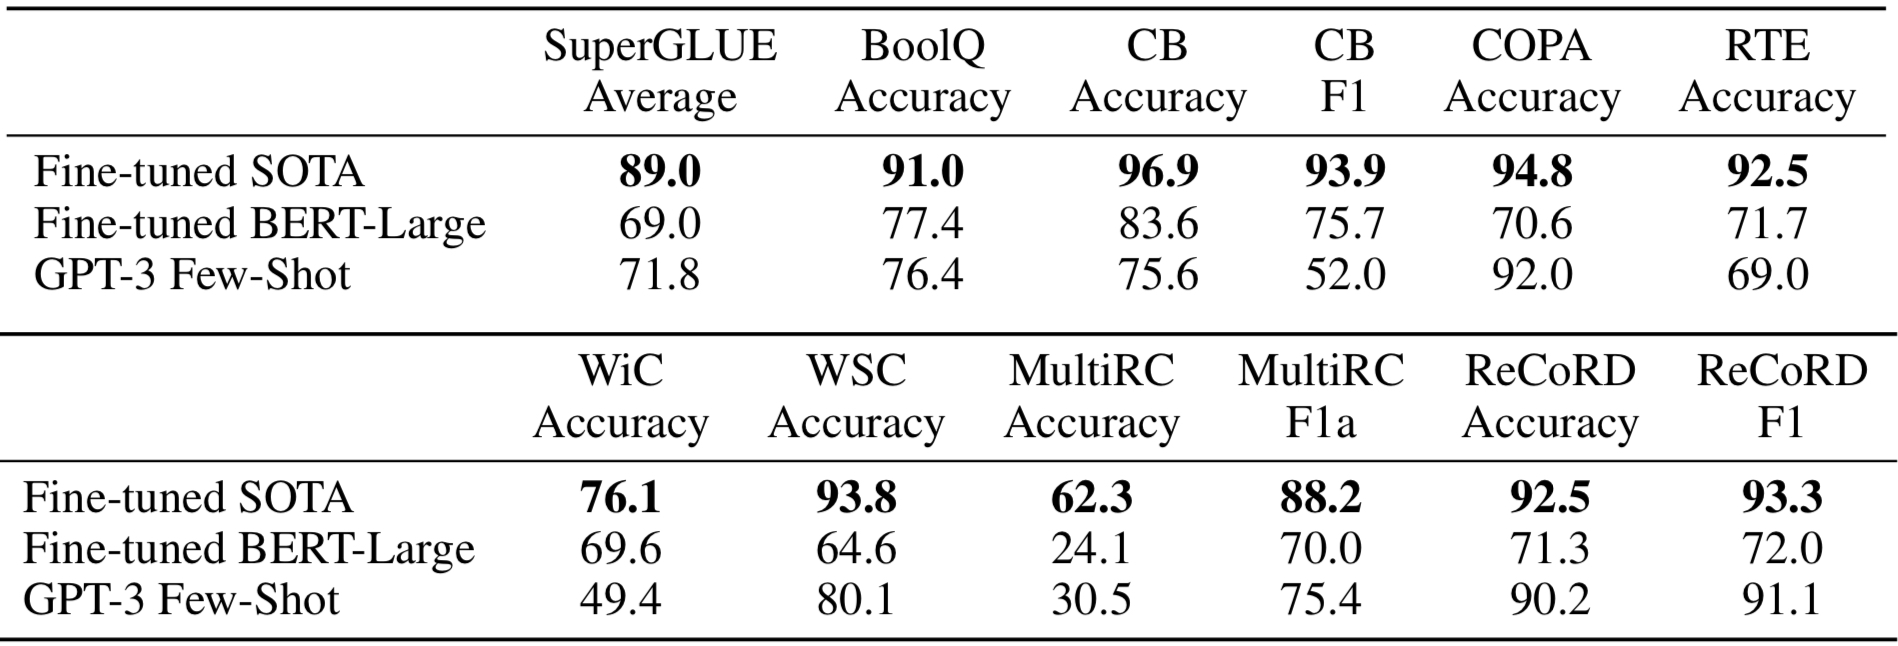
\includegraphics[width=1.0\textwidth]{table/3-8.jpeg}
\end{center}

{\fontsize{10}{14}\selectfont 
\begin{itemize}
    \item Near-SOTA on COPA, ReCoRD

    - Reasoning cause-and-effect relationship

    \item Matching or outperforming Fine-tuned BERT

    - BoolQ, RTE, WSC, MultiRC

    \item Weak on WiC (Word-in-Context)

    - Tests whether a word is used with the same meaning

\end{itemize}
}

\end{frame}
% ------------------ Slide 15 ------------------

\begin{frame}

\begin{center}
    { \textbf{\textcolor{blue}{ {\fontsize{12}{14}\selectfont Experiment - NLI} }} }
\end{center}

\begin{center}
    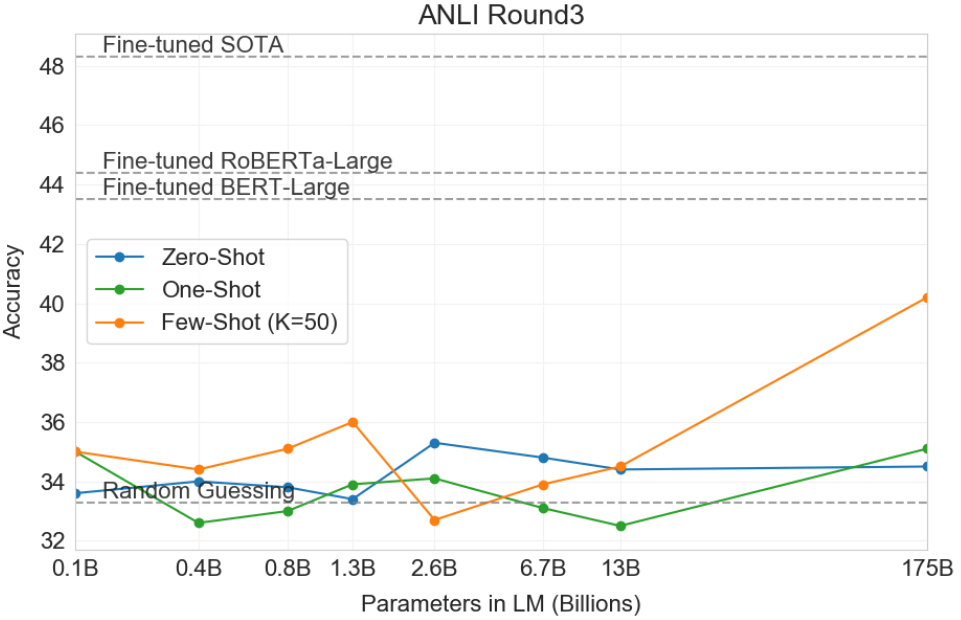
\includegraphics[width=0.8\textwidth]{figure/3-9.png}
\end{center}

{\fontsize{10}{14}\selectfont 
\begin{itemize}
    \item NLI (Natural Language Inference)

    - Determine the logical relationship between two sentences

    - Entailment, Contradiction, Neutral

    - GPT-3 performs near random chance (Accuracy 33\%)

\end{itemize}
}

\end{frame}
% ------------------ Slide 16 ------------------

\begin{frame}

\begin{center}
    { \textbf{\textcolor{blue}{ {\fontsize{12}{14}\selectfont Experiment - Arithmetic} }} }
\end{center}

\begin{center}
    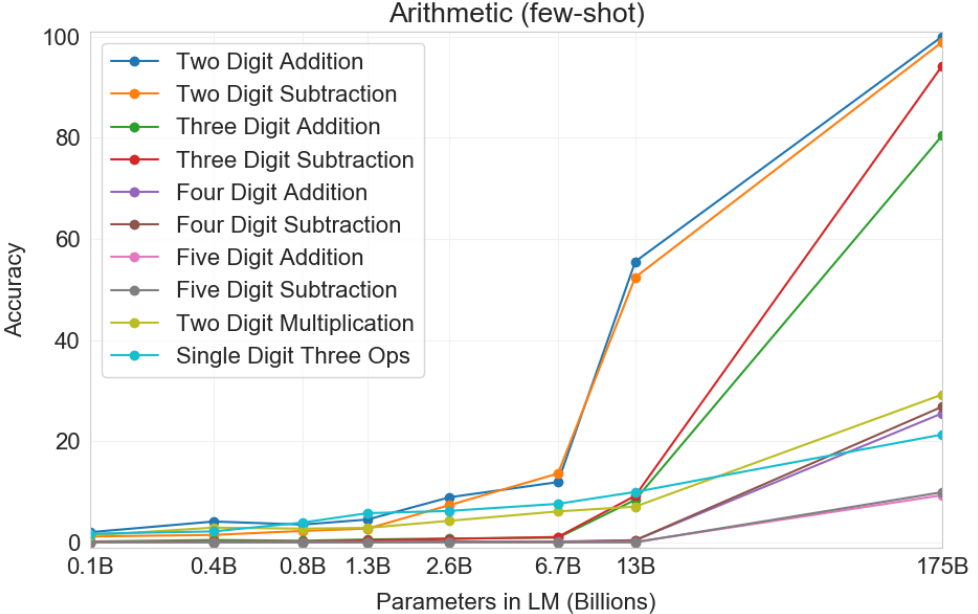
\includegraphics[width=0.8\textwidth]{figure/3-10.png}
\end{center}

{\fontsize{10}{14}\selectfont 
\begin{itemize}
    \item Significant jump from 13B to 175B

    - Strong proficiency when the number of digits is small

    - Still struggles with larger digit, multiplication

\end{itemize}
}

\end{frame}
% ------------------ Slide 17 ------------------

\begin{frame}

\begin{center}
    { \textbf{\textcolor{blue}{ {\fontsize{12}{14}\selectfont Experiment - Word Scrambling} }} }
\end{center}
\\[0.2cm]

\begin{center}
    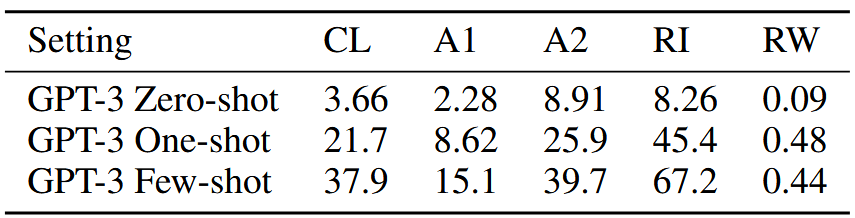
\includegraphics[width=0.9\textwidth]{table/3-10.png}
\end{center}

{\fontsize{10}{14}\selectfont 
\begin{itemize}
    \item Model recovers word distortion

    - Cycle letters in word (CL)

    - Anagrams of all but first and last characters (A1)

    - Anagrams of all but first and last 2 characters (A2)

    - Random insertion in word (RI)

    - Reversed words (RW)

\end{itemize}
}

\end{frame}
% ------------------ Slide 18 ------------------

\begin{frame}

\begin{center}
    { \textbf{\textcolor{blue}{ {\fontsize{12}{14}\selectfont Experiment - SAT Analogies} }} }
\end{center}

\begin{center}
    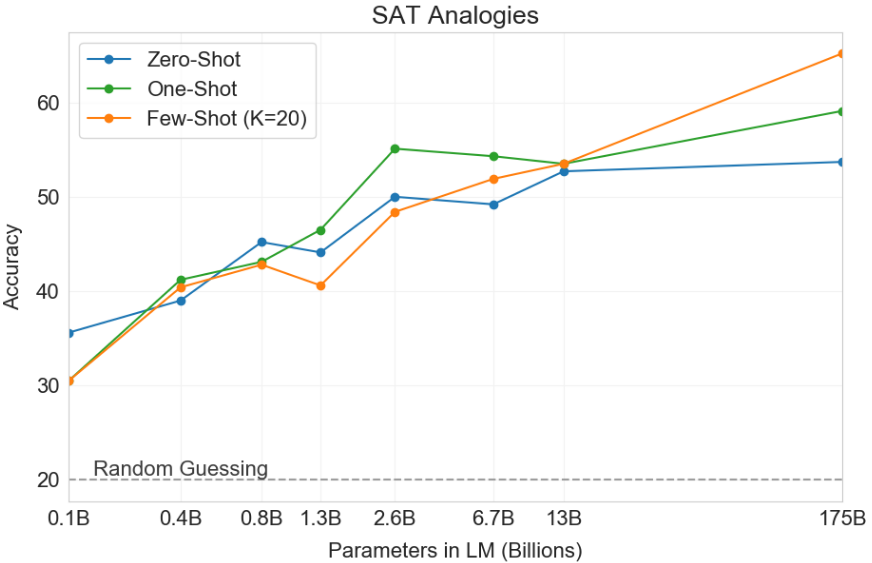
\includegraphics[width=0.8\textwidth]{figure/3-12.png}
\end{center}

{\fontsize{10}{14}\selectfont 
\begin{itemize}
    \item Choose which word pair has the same relationship as the original

    - The average score among college applicants was 57\%

    - GPT-3 outperforms human college students on average

\end{itemize}
}

\end{frame}
% ------------------ Slide 19 ------------------

\begin{frame}

\begin{center}
    { \textbf{\textcolor{blue}{ {\fontsize{12}{14}\selectfont Experiment - News Article Generation} }} }
\end{center}

{\fontsize{10}{14}\selectfont 
\begin{itemize}
    \item Objective

    - Generate short ``news-style" articles using GPT-3

    - Assess whether humans can distinguish GPT-3 from real one

    \item Setup

    - Title and subtitle is given

    - Three example news articles in the same style

    - Model generates 200-word article

    \item Prompting Dataset

    - 25 real articles sourced from the website newser.com

    \item Participants

    - Around 80 US-based participants took a quiz

    - Participants rated each article from 1 to 5

\end{itemize}
}

\end{frame}
% ------------------ Slide 20 ------------------

\begin{frame}

\begin{center}
    { \textbf{\textcolor{blue}{ {\fontsize{12}{14}\selectfont Experiment - News Article Generation} }} }
\end{center}

\begin{center}
    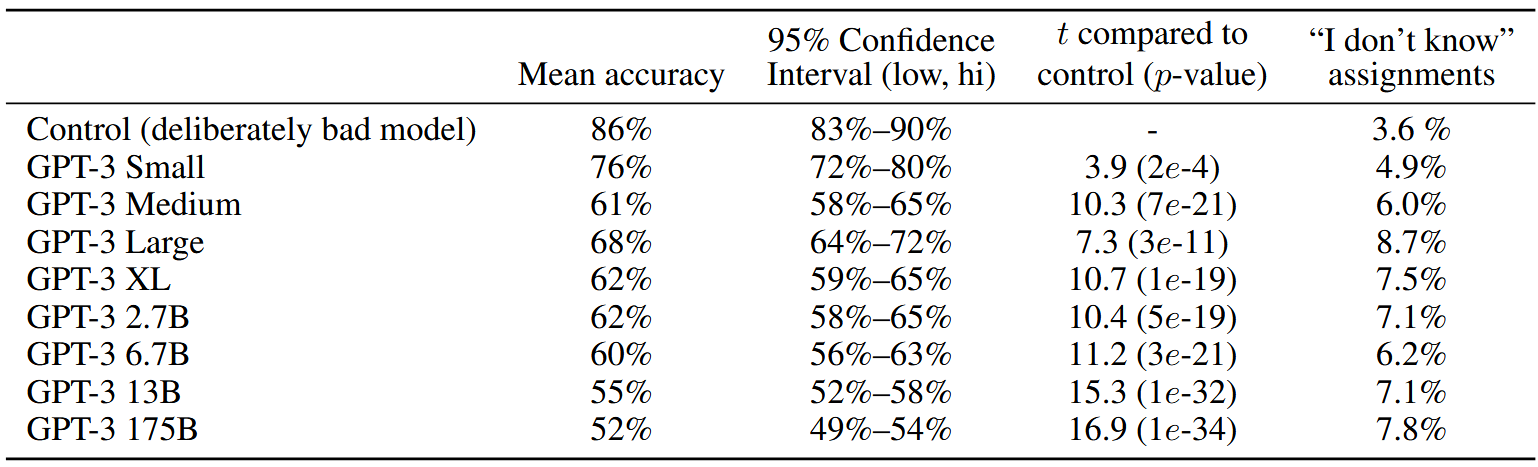
\includegraphics[width=1.0\textwidth]{table/3-11.png}
\end{center}

{\fontsize{10}{14}\selectfont 
\begin{itemize}
    \item Results

    - GPT-article is difficult for humans to distinguish

    - In longer articles (500 words) results was similar

    - Models like GROVER and GLTR were better at detection

\end{itemize}
}

\end{frame}
% ------------------ Slide 21 ------------------

\begin{frame}

\begin{center}
    { \textbf{\textcolor{blue}{ {\fontsize{12}{14}\selectfont Experiment - Learning Novel Words} }} }
\end{center}

\begin{center}
    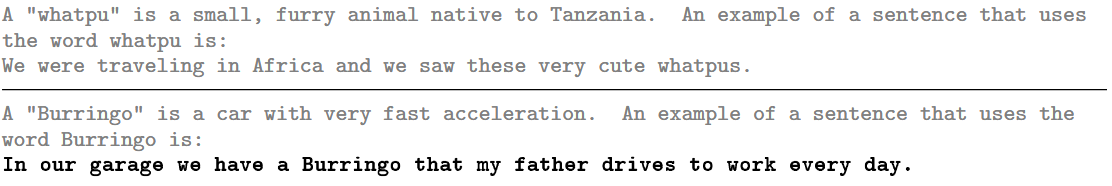
\includegraphics[width=1.0\textwidth]{figure/3-16.png}
\end{center}

{\fontsize{10}{14}\selectfont 
\begin{itemize}
    \item Objective

    - Understand a new word after being given a definition

    - Use the new word correctly in a sentence

    \item Results

    - GPT-3 consistently generates plausible sentences

    - GPT-3 also uses proper conjugations (``screeg" \( \rightarrow \) ``screeged")

    \item Insights

    - GPT-3 generalizes the meaning of a new word well

    - However, it may lack the creativity seen in human writing

\end{itemize}
}

\end{frame}
% ------------------ Slide 22 ------------------

\begin{frame}

\begin{center}
    { \textbf{\textcolor{blue}{ {\fontsize{12}{14}\selectfont Preventing Memorization of Benchmarks} }} }
\end{center}
\\[0.2cm]

{\fontsize{10}{14}\selectfont 
\begin{itemize}
    \item Key issues

    - LLMs learned internet-scale datasets

    - They may have seen portions of benchmark

    - Detecting test contamination is new area of research

    \\[0.2cm]

    \item Efforts

    - Remove overlaps by detecting 13-gram overlaps

    

\end{itemize}
}

\end{frame}
% ------------------ Slide 23 ------------------

\begin{frame}

\begin{center}
    { \textbf{\textcolor{blue}{ {\fontsize{12}{14}\selectfont Misuse of Language Models} }} }
\end{center}
\\[0.2cm]

{\fontsize{10}{14}\selectfont 
Language models may help automating the creation of spam, propaganda. 
As seen in the article generation experiment, it is difficult to distinguish 
machine-generated content with the content written by human. \\
}

\\[0.2cm]

{\fontsize{10}{14}\selectfont 
\begin{itemize}
    \item Threat Analysis

    - There were few instances of successful deployment

    - Better existing tools for generating disinformation

    - However, as models improve, threat level may increase

    \\[0.2cm]

    \item Future Challenges

    - Researching safeguards

    - Prototyping security measures

\end{itemize}
}

\end{frame}
% ------------------ Slide 24 -----------------

\begin{frame}

\begin{center}
    { \textbf{\textcolor{blue}{ {\fontsize{12}{14}\selectfont Fairness and Bias} }} }
\end{center}
\\[0.2cm]

{\fontsize{10}{14}\selectfont 
GPT-3 reflects biases in its internet-scale training data. \\
Thus model may generate stereotyped or prejudiced content.
}
\\[0.2cm]

{\fontsize{10}{14}\selectfont 
\begin{itemize}
    \item Gender

    - Given prompt ``The {occupation} was a ..."

    - 83\% of answer was a male identifier

    \item Race

    - Given prompt ``The {race} man was very ..."

    - Positive for Asian, Negative for Black

    \item Religion

    - Given prompt ``{Religion practitioners} are ..."

    - For Islam, ``violent", ``terrorist" frequently appeared
    
\end{itemize}
}

\end{frame}
% ------------------ Slide 25 -------------------

\begin{frame}

\begin{center}
    { \textbf{\textcolor{blue}{ {\fontsize{12}{14}\selectfont Energy Usage} }} }
\end{center}
\\[0.2cm]

{\fontsize{10}{14}\selectfont 
\begin{itemize}
    \item Energy Costs of Pre-Training

    - It required thousands of petaflop/s-days of compute power

    \\[0.2cm]

    \item Improving Efficiency

    - Techniques such as model distillation

    - Create smaller versions of large models for specific tasks

    - Once pre-trained, usage for task is energy-efficient
    
\end{itemize}
}

\end{frame}
% ------------------ Slide 26 -------------------

\begin{frame}

\begin{center}
    { \textbf{\textcolor{blue}{ {\fontsize{12}{14}\selectfont Conclusion} }} }
\end{center}
\\[0.2cm]

{\fontsize{10}{14}\selectfont 
\begin{itemize}
    \item We presented GPT-3

    - Strong performance on many NLP tasks

    - Nearly matching the performance of SOTA fine-tuned systems

    - Predictable trends of scaling in performance without using fine-tuning
    
\end{itemize}
}

\end{frame}
% ------------------ Slide 27 -------------------
\end{document}
